

\section{Method}
\label{sec:methods}

We first describe our classifier for detecting split errors which is based on a convolutional neural network (CNN). We detail the CNN architecture, input features and the training method. We then describe how the same classifier can be used to detect merge errors and how we create potential corrections. The classifiers are integrated into an existing proofreading workflow as reported after. Finally, we explore an active label suggestion method which reorders the ranking obtained by our classifiers and maximizes the information gain provided by each potential correction.

\subsection{Split Error Detection}

We build a split error classifier with output $p$ using a convolutional neural network (CNN) to check whether an edge within an existing automatic segmentation is valid ($p=0$) or not ($p=1$). Rather than analyzing every input pixel, the classifier operates only on segment boundaries which requires less pixel context and is faster. Our approach was inspired by Bogovic \etal~\cite{BogovicHJ13} but works with 2D slices rather than 3D volumes. This enables proofreading prior or in parallel to an expensive alignment of individual EM images.
\\~\\
\textbf{Convolutional Neural Network Architecture.} Split error detection of a given boundary is really a binary classification task since the boundary is either correct or erroneous. However, in reality the score $p$ is between 0 and 1. The classification complexity arises from hundreds of different cell types in connectomics data rather than from the classification decision. Intuitively, this yields a wider (meaning more filters) rather than a deeper (meaning more layers) architecture. We explored different architectural configurations - including residual networks~\cite{resnet} - by performing a brute force parameter search and comparing precision and recall (see supplementary materials). Our final CNN configuration for split error detection is composed of four convolutional layers, each followed by max pooling as well as dropout regularization to prevent overfitting due to limited training data. Fig. \ref{fig:architecture} shows the CNN architecture for split error detection.
\\~\\
\textbf{Classifier Inputs.} To train the CNN for split error detection, we take boundary context information into consideration for the decision making process. For this, we grab a $75x75$ pixel patch at the center of an existing boundary. This covers approximately $80\%$ of all boundaries in real-world connectomics data with nanometer resolution. If the boundary edge is not fully covered, we sample up to 10 non-overlapping patches along the boundary and combine the resulting score by weighted averaging based on boundary length coverage per patch. In their paper, Bogovich \etal propose to use grayscale image data, corresponding boundary probabilities, and  a single binary mask combining the two neighboring labels as features for their recursive neural network~\cite{BogovicHJ13}. We are building on this set of features as inputs for our CNN and create a stacked pixel patch. However, we observed that the boundary probability information generated from EM images is often misleading due to noise or artefacts in the data. This can result in merge errors within the automatic segmentation. To better direct our classifier to train on the true boundary edge, we extract the border between two segments. We then dilate this border by 5 pixels to consider slight edge ambiguities and use this additional binary mask as another feature to create a 4-channel input patch. Fig. \ref{fig:cnn_inputs} shows examples of correct and erroneous feature patches and their corresponding automatic segmentation and ground truth. 

\begin{figure}[h]
\begin{center}
  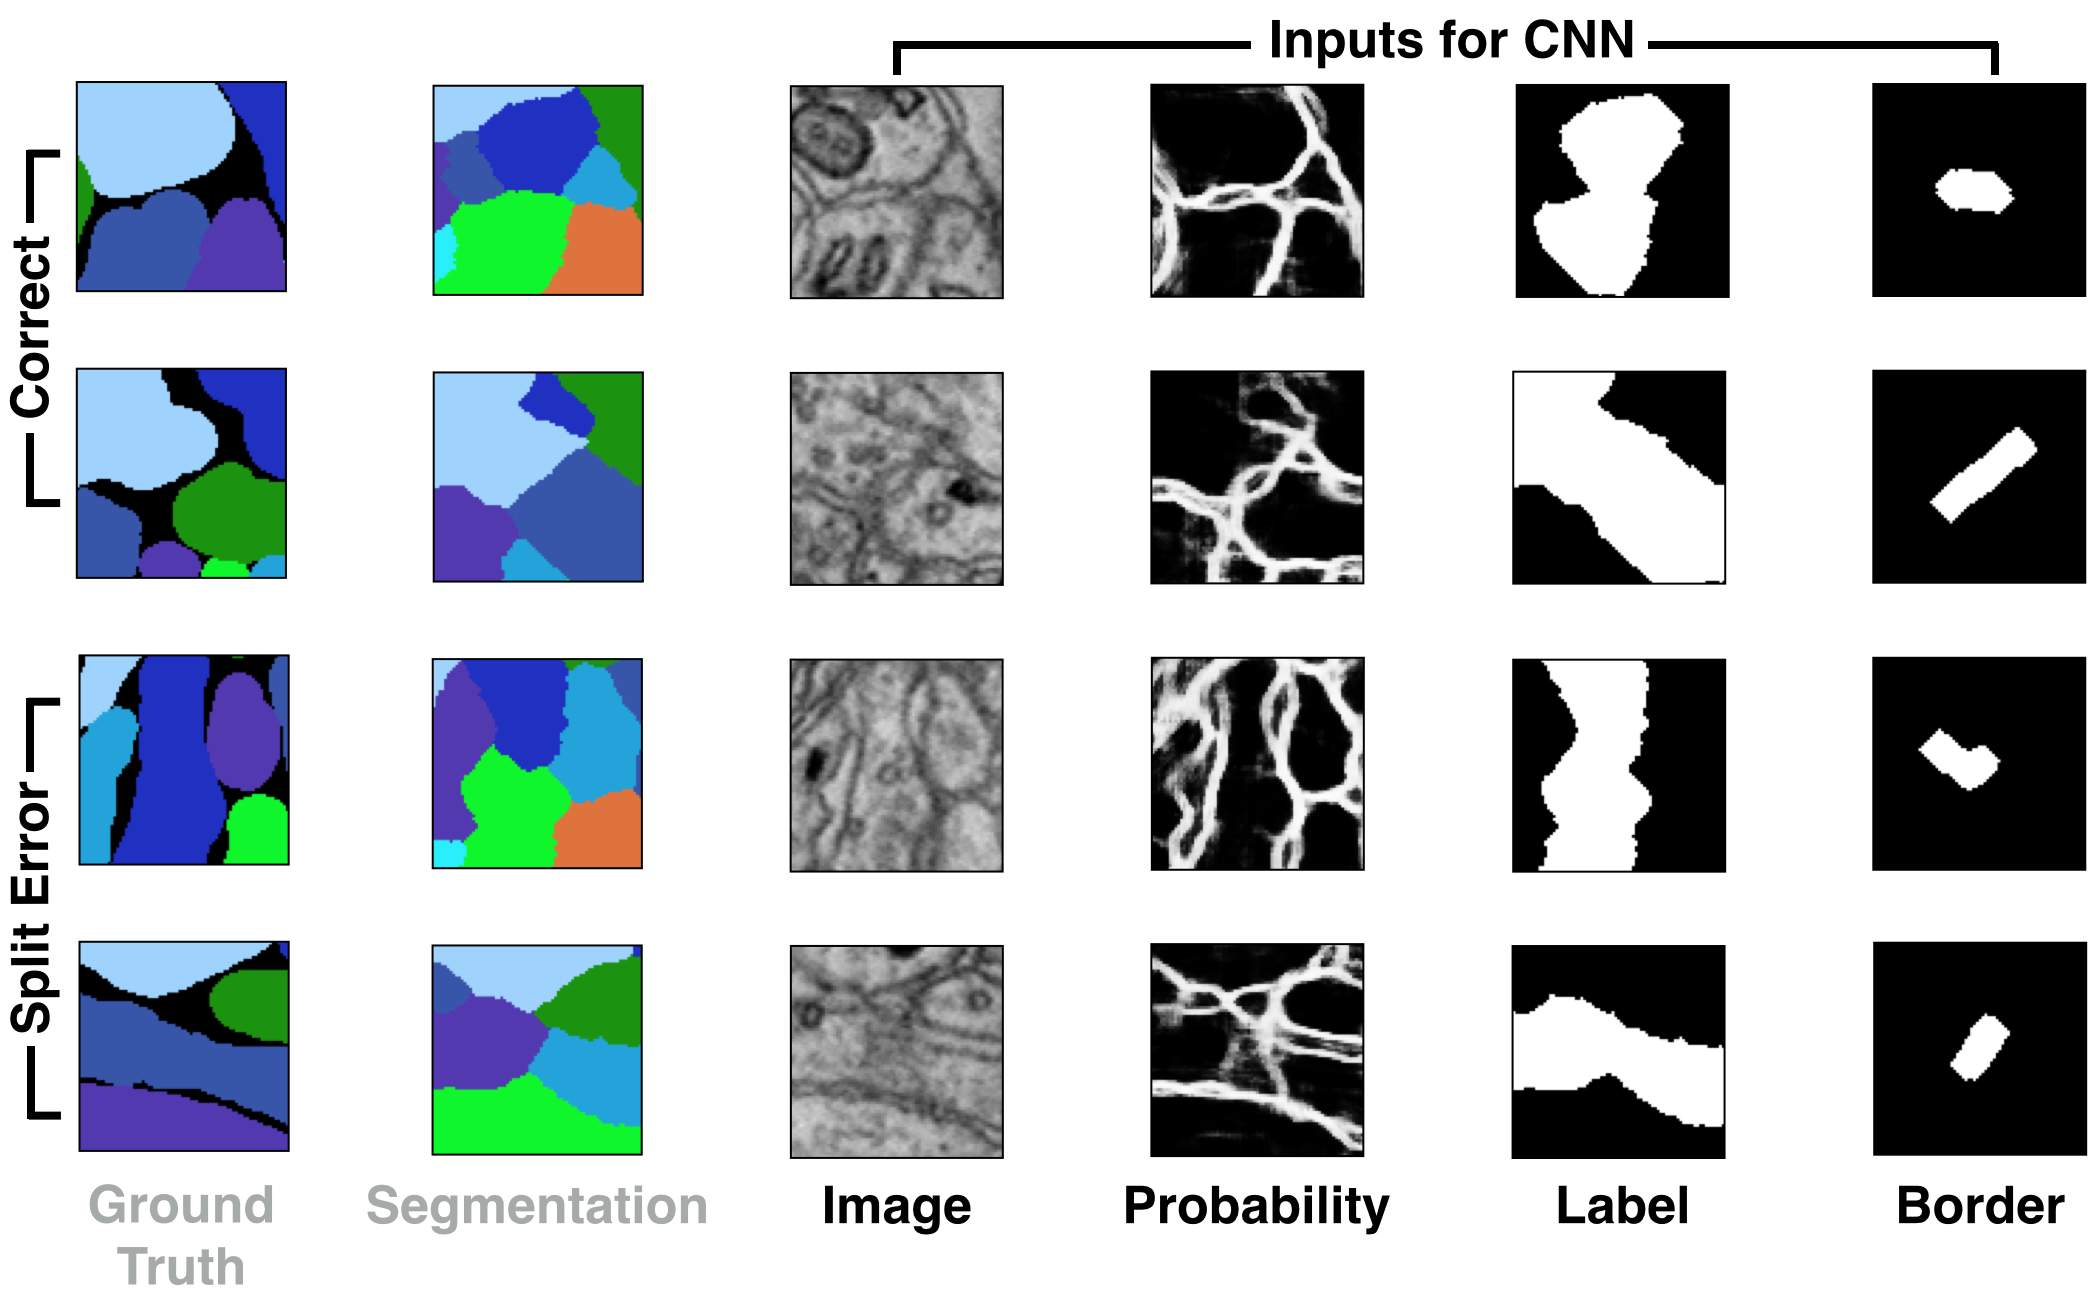
\includegraphics[width=\linewidth]{gfx/cnn_inputs.png}
\end{center}
  \vspace{-4mm}
   \caption{Example inputs for learning correct splits and split errors as reflected in the segmentation relative to the ground truth. Image, membrane probabilities, merged binary labels, and a dilated border mask are combined to 4-channel input patches.}
\label{fig:cnn_inputs}
\end{figure}

\textbf{Training.} To initially train our network, we use the blue 3-cylinder mouse cortex volume of Kasthuri \etal~\cite{kasthuri2015saturated} ($2048\times2048\times300$ voxels). The tissue is dense mammalian neuropil from layers 4 and 5 of the S1 primary somatosensory cortex of a healthy mouse. The resolution of our dataset is $3\, nm$ per pixel, and the section thickness is $30\, nm$. The image data and a manually-labeled expert segmentation is publicly available as ground truth for the entire dataset\footnote{The Kasthuri 3-cylinder mouse cortex volume is available at  https://software.rc.fas.harvard.edu/lichtman/vast/}. We use the first 250 sections of the data for training and validation and the last 50 for testing. We use a state-of-the-art method to create a dense automatic segmentation of the data. To generate training data, we identify correct regions and split errors in the automatic segmentation by intersection with ground truth regions. This is required since extracellular space is not labeled in the ground truth but in our dense automatic segmentation. From these regions, we sample 120,000 correct and 120,000 split error patches with 4-channels as described above. The patches are normalized and to further augment our training data, we rotate patches within each mini-batch by $k*90$ degrees with randomly chosen $k$. The training parameters such as filter size, number of filters, learning rate, and momentum are the result of intuition and experience, studying recent machine learning research as well as a brute force parameter search within a limited range (see supplementary material). The final parameters and training results are listed in table~\ref{tab:parameters}. For baseline comparison, we also list the parameters and training results of focused proofreading in this table but elaborate on these further in section \ref{sec:evaluation}. Our CNN configuration results in approximately 170,000 learnable parameters. We assume that training has converged if the validation loss does not decrease for 50 epochs.

\begin{table}[h]
%\resizebox{\textwidth}{!}{%
\tiny
\begin{tabular}{@{}c|c|c|c|c|c|c@{}}
& \textbf{cost [m]} & \textbf{Val. loss} & \textbf{Val. acc.} & \textbf{Test acc.} & \textbf{Prec./Recall} & \textbf{F1 Score} \\ 
\hspace{1mm}
\begin{tabular}{@{}l@{}}
\textbf{Guided Proofreading} \\ Filter size: 3x3 \\ No. Filters 1: 64 \\ No. Filters 2-4: 48 \\ Dense units: 512 \\ Learning rate: 0.03-0.00001\\ Momentum: 0.9-0.999\\Mini-Batchsize: 128\\~\\
 \end{tabular}
 & 383  & 0.0845  & 0.969  & 0.94  & 0.94/0.94  & 0.94 \\ 
\hline 
\begin{tabular}{@{}l@{}}
\\
\textbf{Focused Proofreading} \\ 
Iterations: 3 \\
Learning strategy: 2\\
Mito agglomeration: Off\\
Threshold: 0.2
 \end{tabular}
 & 43  & ?  & ?  & 0.839  & ?/?  & ? \\ 
\end{tabular} 
\vspace{1mm}
\caption{Training parameters, cost and results of our guided proofreading classifier versus focused proofreading by Plaza \cite{focused_proofreading}. Both methods were trained on the same mouse brain dataset using the same hardware (Tesla K40 graphics card). While the training of our classifier is more expensive, testing accuracy is superior. }
\label{tab:parameters}
\end{table}

For performance comparison on data of a different species, in particular on fruitfly brain (drosophila), we retrain our network. The training procedure is according to our initial training and network architecture as well as parameters are not changed. We further elaborate on the drosophila datasets in section~\ref{sec:evaluation}. Fig.~\ref{fig:roc} displays receiver operating characteristics (ROC) for  guided proofreading trained on mouse and drosophila data, as well as our comparison baseline focused proofreading trained on these datasets respectively.

\begin{figure}[h]
  \vspace{-5mm}
\begin{center}
  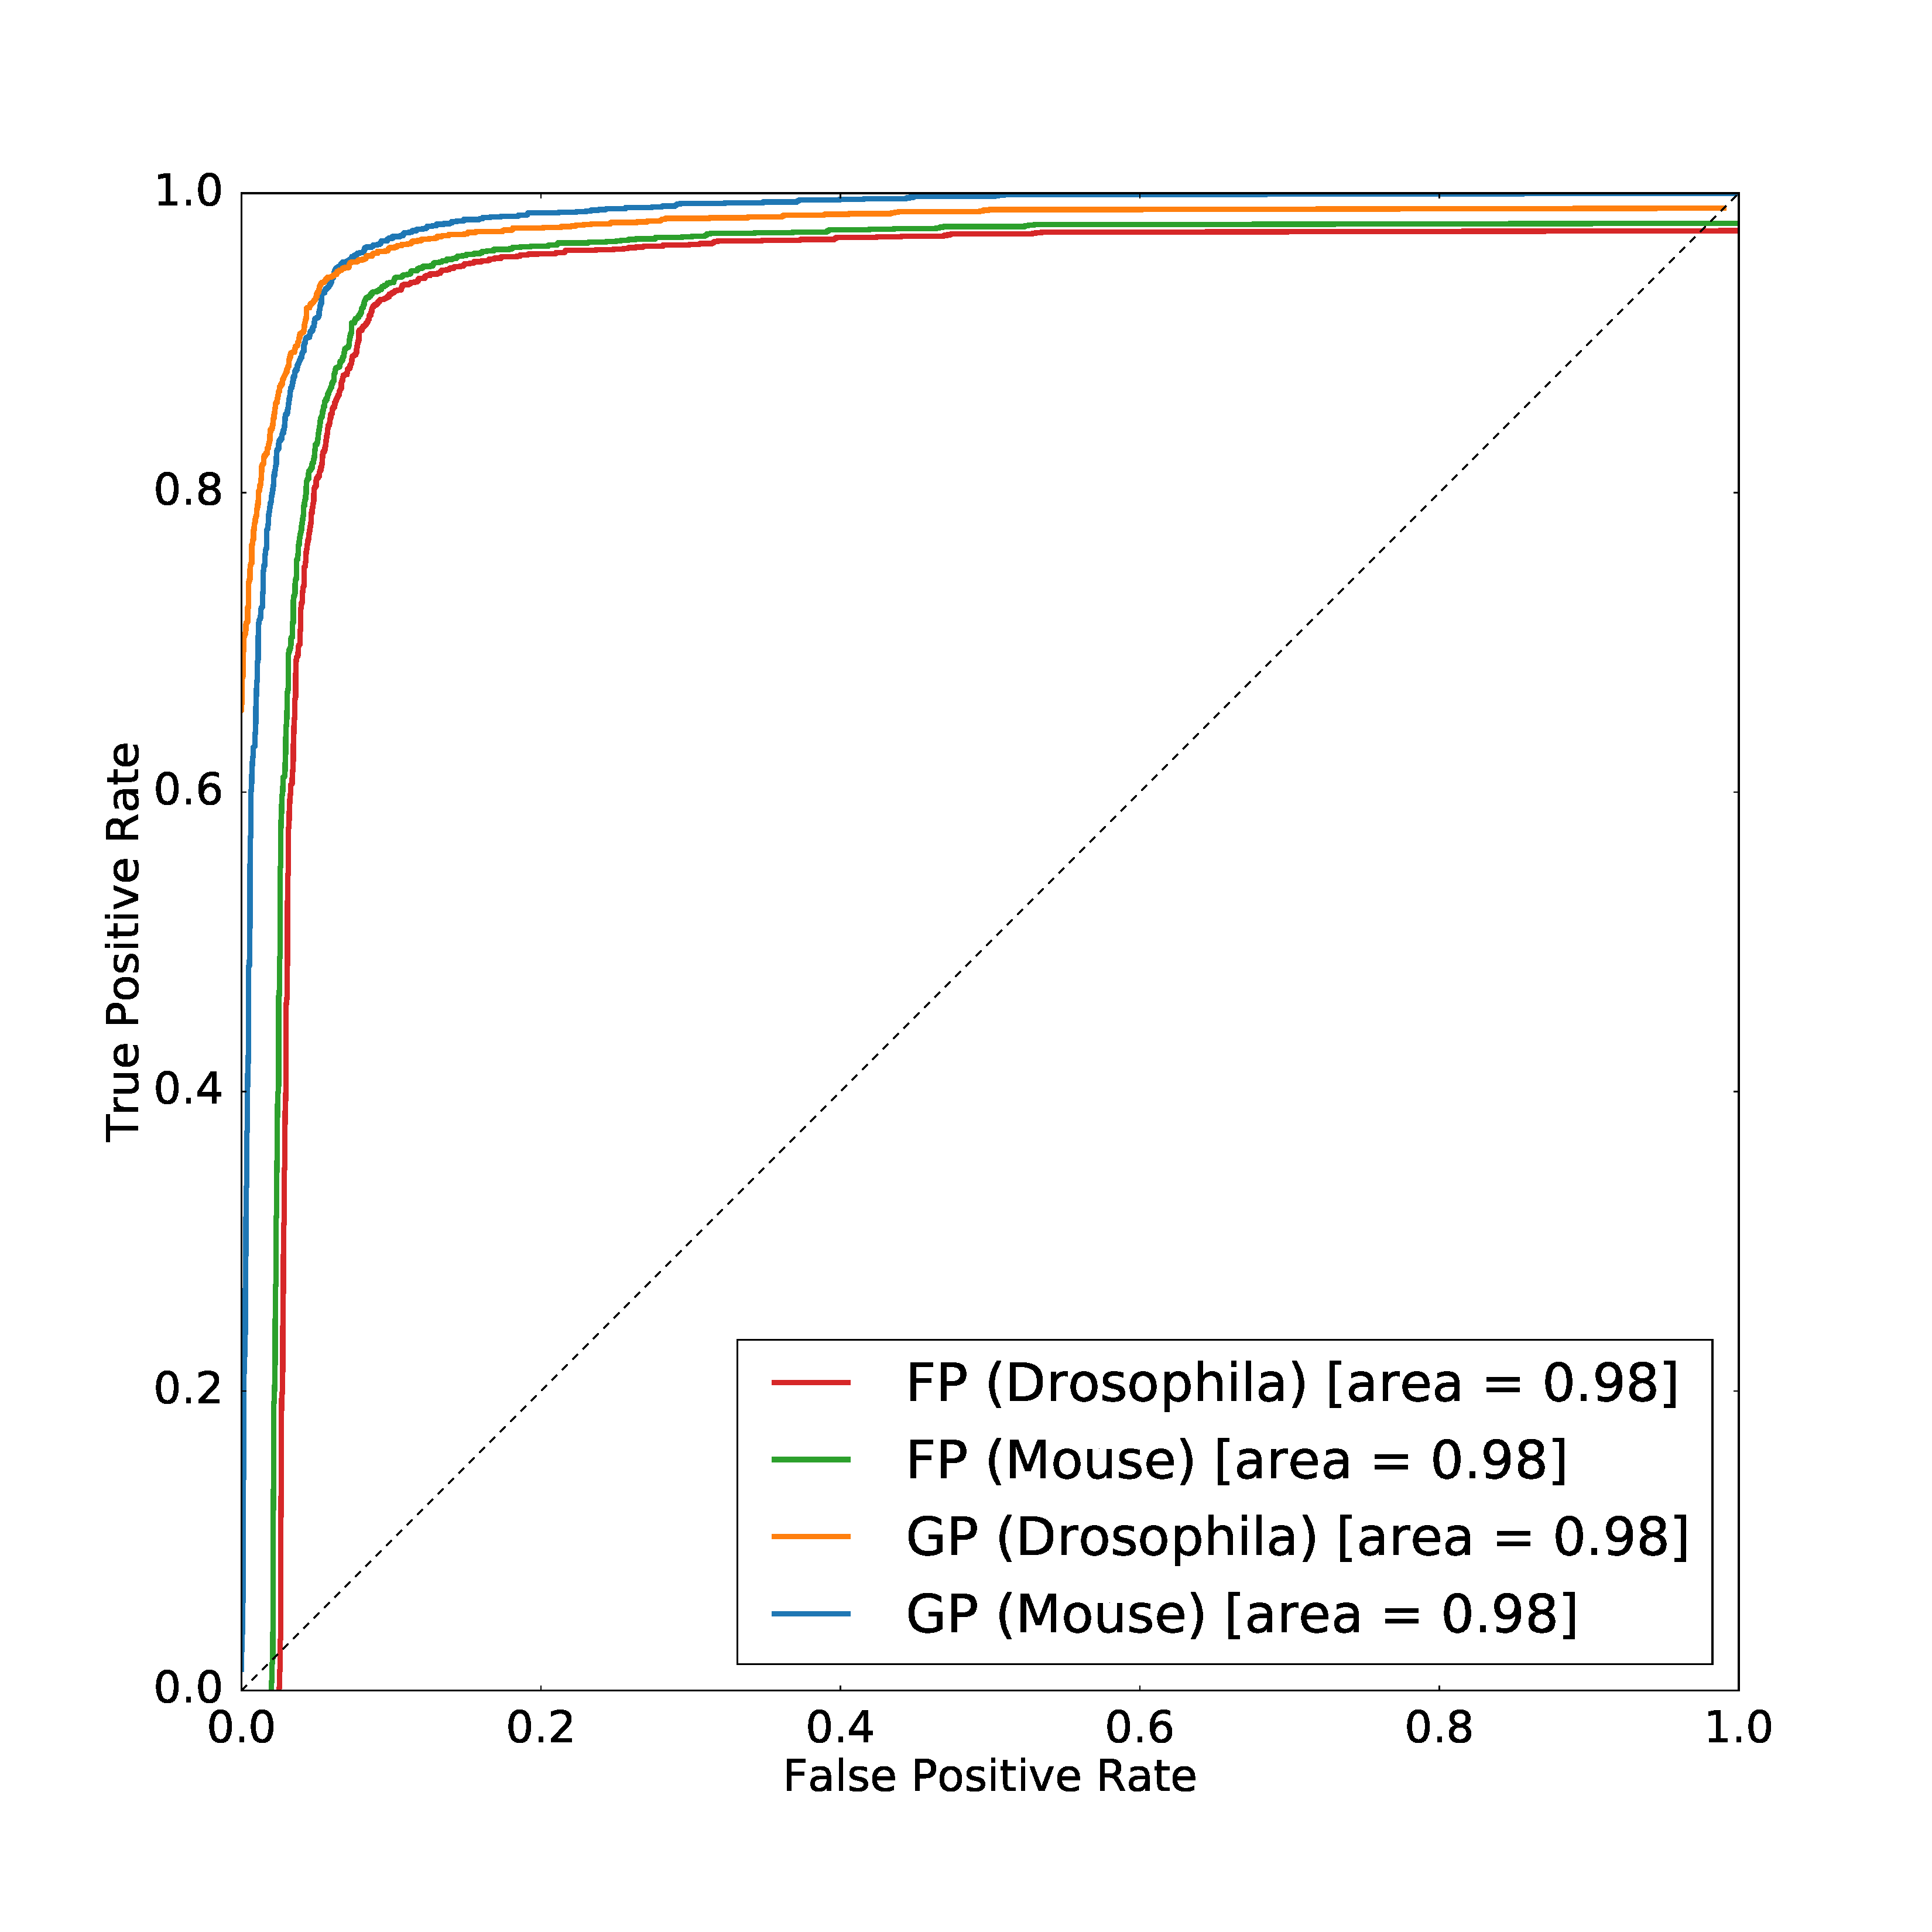
\includegraphics[width=\linewidth]{gfx/roc.pdf}
\end{center}
  \vspace{-10mm}
   \caption{ROC performance of guided proofreading (GP) and focused proofreading (FP) trained separately on mouse and drosophila brain images. The area under the curve indicates better performance for GP.}
\label{fig:roc}
\end{figure}
 

\subsection{Merge Error Detection}

Identification and correction of merge errors is more challenging, because we must look inside segmentation regions for missing or incomplete boundaries and then propose the correct boundary. However, we can reuse the same trained CNN for this task. Similar to guided volume editing by Karimov~\etal~\cite{karimov_guided_volume_editing} we generate potential borders within a segment. For each segmentation label, we dilate the label by 20 pixel and generate 30 potential boundaries through the region by randomly placing watershed seed points at opposite sides of the label boundary. For watershed, we use the inverted gray scale EM image as features. This yields 30 corresponding splits. Dilation of the segment prior to watershed is motivated by our observation that the generated split then actually hogs the real membrane boundary. These boundaries are then individually rated using our split error classifier. For this, we invert the probability score meaning that a correct split (previously encoded as $p=0$) is most likely a candidate for a merge error (now encoded as $p=1$). In other words, if a generated boundary is ranked as correct, it probably should be in the segmentation. Fig. \ref{fig:merge_error} illustrates this procedure.

\begin{figure}[h]
\begin{center}
  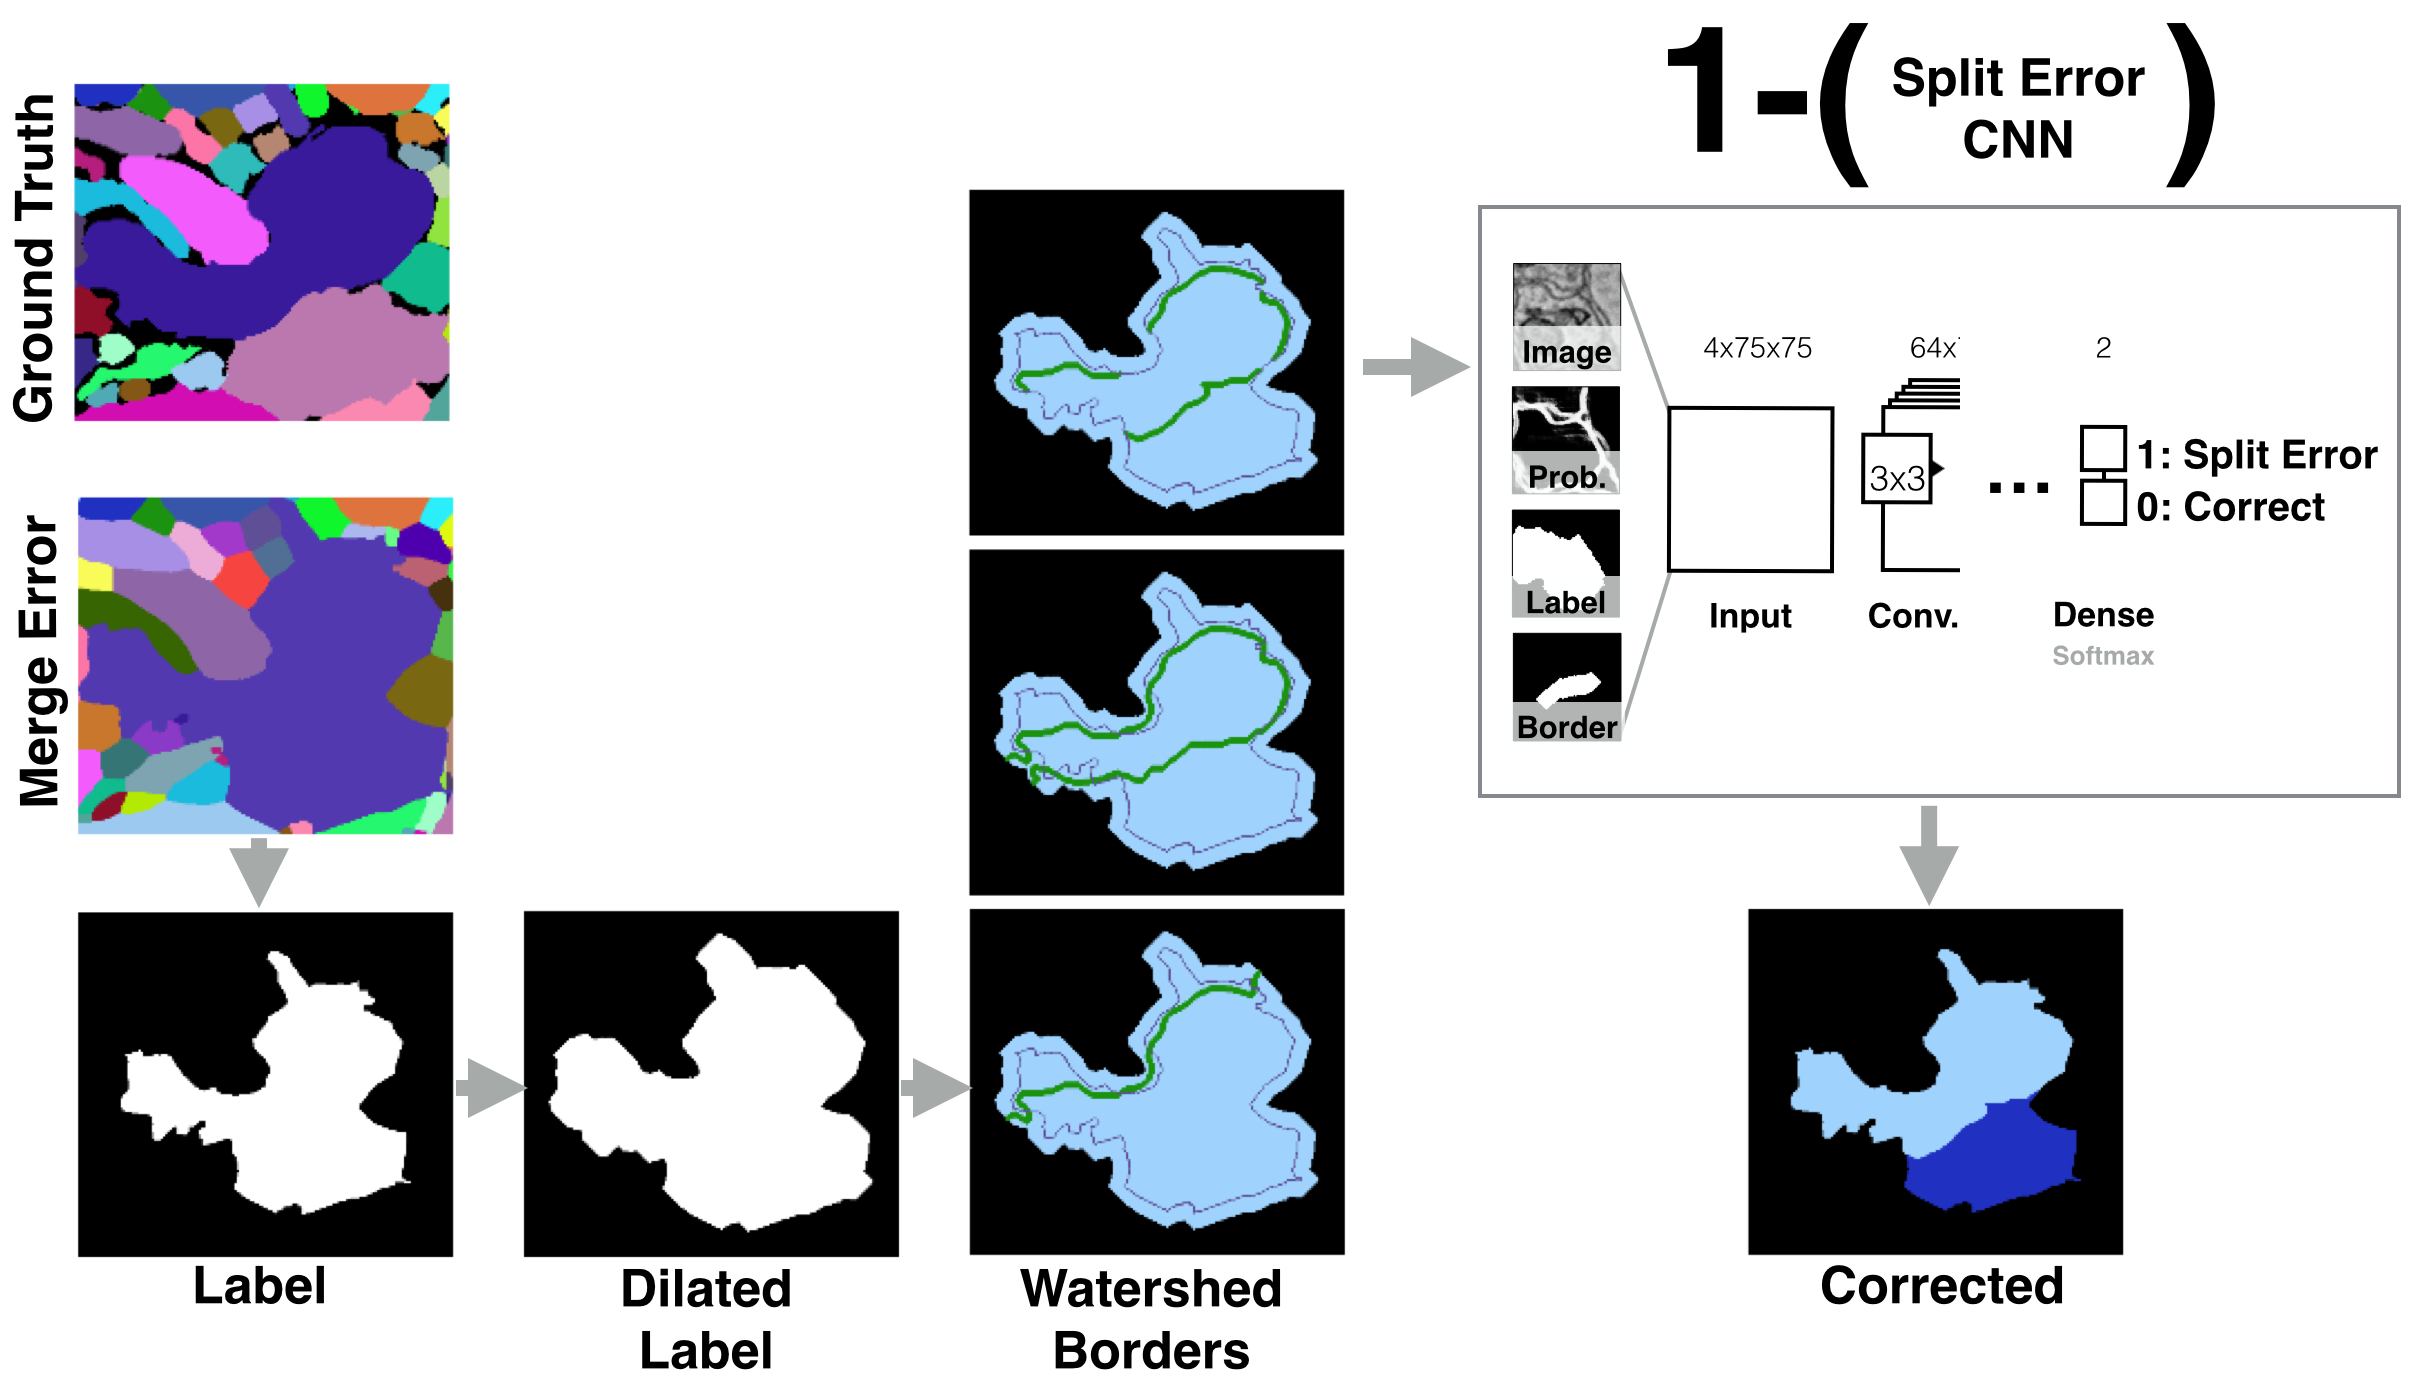
\includegraphics[width=\linewidth]{gfx/merge_error.png}
\end{center}
  \vspace{-4mm}
   \caption{Merge errors are identified by generating randomly seeded watershed borders within a dilated label segment. These borders then are individually rated using the split error CNN by inverting the probability score. This way, a confident rating for a correct split most likely indicates the missing border of the merge error and can be used for correcting the labeling.}
\label{fig:merge_error}
\end{figure}

\subsection{Error Correction}

We use the proposed classifiers in combination to perform corrections of split and merge errors in automatic segmentations. For this, we first perform merge error detection for all existing segments in a data set and store the inverted ranking $1-p$. We then sort the rankings and loop through all of them in greedy fashion, starting with the most likely error. If the inverted score $1-p$ of a merge error is higher than a threshold $p_t$, we mark this merge error for correction. The merge error detection yields the potential new boundary and we can modify the segmentation data to create a new segment accordingly. Depending on the variation of guided proofreading as described in section~\ref{sec:evaluation}, we either perform the correction directly (automatic GP) or we have a user accept or reject the correction (simulated GP or human novice/expert).
Once all merge errors are corrected, we perform split error detection. For this, we perform split error detection and store the ranking $p$ for all existing segments in the for merge errors corrected segmentation. We then sort the rankings and again loop through all of them - the most likely error first. If the score $p$ is higher than a threshold $p_t$, we mark the split error for correction. Potential split errors are identified at the border of two segments. This reduces the correction to merging the segments and is therefore trivial. Similarly to merge errors, we either perform the correction directly or present a user with a yes/no decision. Our experiments have shown that the threshold $p_t$ is the same for merge and split errors which makes sense for a balanced classifier. The only exception is when a user drives the correction process: we then set $p_t$ for split errors to 0 to let the user inspect every possible split error. Inspecting all merge errors is not possible for users due to the sheer amount of generated borders.

\subsection{Application}

Guided proofreading is integrated into an existing workflow for large connectomics data. The GP system is web-based and is designed with a minimalistic user interface showing three components. First, we show the outline of the current labeling of a cell boundary and its proposed correction on top of the EM image data. For the user, it is not possible to distinguish the current labeling and the proposed correction to avoid selection bias. Second, we show a solid overlay of the current and proposed labeling. And finally, to provide context, we show a larger area of the EM image where the potentially erroneous region is highlighted. User interaction is simple and involves one mouse click on either the current labeling or the correction. After interaction, the next potential error is shown. We provide a screenshot of the application as part of the supplementary material.

\subsection{Active Label Suggestion}

In an interactive setting, one way to present patches to the user for proofreading is to order them by the confidence probability of the GP classifier. However, in an active learning setting, where the network is retrained repeatedly on new label evidence, this approach is less likely to decrease segmentation error as, with the new labels, we are only reinforcing what the network already has a high confidence in.
Instead, we apply active label suggestion to guide the user into labeling patches which will be more informative to retraining, and so overall decrease VI faster within the proofreading cycle of label $\rightarrow$ train $\rightarrow$ label. For each patch, we remove the softmax classification layer and look at the activation weights associated with the last dense layer. These become a high-dimensional feature vector. Then, we adapt Anon~\etal~\cite{ANON} to provide label suggestions based on features from the learned CNN, which is based on maximizing the average information gain provided by a candidate patch to label.
A second consideration is that each patch labeled by the user provides evidence to other patches, e.g., correcting a split error redefines an entire boundary, from which multiple candidate patch labelings could have been drawn. As such, when the user labels a patch, we consider all `knock-on' effect patches as also being labeled, and feed these into the active label suggestion system similarly.
In section \ref{sec:evaluation}, we report the difference in performance from using active label suggestion rather than confidence ordering when presenting patches to the user. These results are without retraining the network after new labelings: this should improve results, but would have to be batched to reduce computational load; hence, we leave this for future work.

 